\documentclass{beamer}

\usepackage{minted}

\usepackage{tikz}
\usetikzlibrary{patterns}
\usetikzlibrary{calc}
\usetikzlibrary{shapes, arrows, positioning}

\usepackage{tabularray}
\UseTblrLibrary{booktabs}
\DefTblrTemplate{contfoot-text}{normal}{\lang{(Continued on next page)}{(Continua na próxima página)}} 
\SetTblrTemplate{contfoot-text}{normal} 
\DefTblrTemplate{conthead-text}{normal}{\lang{(continued)}{(continuação)}} 
\SetTblrTemplate{conthead-text}{normal}

\usepackage{enumitem}
\definecolor{ifscgreen}{RGB}{50,93,61}

\setlist[enumerate,1]{label=\colorbox{ifscgreen}{\textcolor{white}{\arabic*}}\quad, leftmargin=*}
\setlist[enumerate,2]{label=\colorbox{ifscgreen!70}{\textcolor{white}{\arabic{enumi}.\arabic*}}\quad, leftmargin=*}
\setlist[enumerate,3]{label=\colorbox{ifscgreen!40}{\textcolor{white}{\arabic{enumi}.\arabic{enumii}.\arabic*}}\quad, leftmargin=*}
% ------------------------------
% Codificação e idioma
% ------------------------------
% \usepackage[utf8]{inputenc}
\usepackage[T1]{fontenc}
\usepackage[brazil]{babel}

% ------------------------------
% Matemática e símbolos
% ------------------------------
\usepackage{amsmath}

% ------------------------------
% Gráficos e figuras
% ------------------------------
\usepackage{graphicx}
\usepackage{subfigure}

% ------------------------------
% Cores, URL e hiperlinks
% ------------------------------
\usepackage{url,color}
\usepackage{hyperref}
\hypersetup{
  pdfstartview={Fit},
  pdftitle={\@title},
  pdfsubject={Engenharia de Telecomunicacoes - IFSC},
  pdfauthor={\@author}
}

% ------------------------------
% Listagens e pseudocódigo
% ------------------------------
\usepackage[
plainruled,
noline
]{algorithm2e}

% ------------------------------
% Bibliografia
% ------------------------------
\usepackage[backend=biber,style=numeric,citestyle=ieee]{biblatex}
\addbibresource{references.bib}
\setbeamertemplate{bibliography item}{\insertbiblabel}

% ------------------------------
% Outros pacotes
% ------------------------------
\usepackage{ifsc} % (pacote personalizado, ok manter)

% ------------------------------
% Macros e comandos personalizados
% ------------------------------
\newcommand{\tab}[1]{\hspace{.2\textwidth}\rlap{#1}}

\newcommand{\DAY}{\the\day}
\newcommand{\MONTH}{%
  \ifcase\the\month
  \or Janeiro%
  \or Fevereiro%
  \or Março%
  \or Abril%
  \or Maio%
  \or Junho%
  \or Julho%
  \or Agosto%
  \or Setembro%
  \or Outubro%
  \or Novembro%
  \or Dezembro%
  \fi}
\newcommand{\YEAR}{\the\year}

% ------------------------------
% Dados do título
% ------------------------------
\title{PRG203402 - Lógica de Programação:}
\subtitle{\LARGE Estruturas de decisão e repetição}
\author{João Cláudio Elsen Barcellos}
\date{\scriptsize \DAY~de \MONTH~de \YEAR}
\institute{
  Engenheiro Eletricista\\
  Formado na Universidade Federal de Santa Catarina\\
  campus Florianópolis\\
  \url{joaoclaudiobarcellos@gmail.com}
}

% ------------------------------
% Customização das seções no Beamer
% ------------------------------
\def\sectionname{}
\def\insertsectionnumber{}
\def\subsectionname{}
\def\insertsubsectionnumber{}

\AtBeginSection[]{
  \begin{frame}
      \vfill
      \centering
      \begin{beamercolorbox}[sep=8pt,center,shadow=true,rounded=true]{title}
          \usebeamerfont{title}\insertsectionhead\par%
      \end{beamercolorbox}
      \vfill
  \end{frame}
}

\setbeamertemplate{caption}[numbered]

% ------------------------------
% Controle de idioma
% ------------------------------
\usepackage{ifthen}
\newboolean{english}
\setboolean{english}{false} % true = inglês, false = português

% Configuração de idioma e títulos
\ifthenelse{\boolean{english}}{
  \usepackage[english]{babel}
  \renewcommand{\figurename}{Figure}
  \renewcommand{\tablename}{Table}
  \SetAlgorithmName{Algorithm}{}{}
  
  \SetKwInput{KwData}{Input}
  \SetKwInput{KwResult}{Output}
  \SetKwIF{If}{ElseIf}{Else}{if}{then}{else if}{else}{end if}
  \SetKwFor{While}{while}{do}{end while}
  \SetKwFor{For}{for}{do}{end for}
  \SetKw{Return}{return}
}{
  \usepackage[brazil]{babel}
  \renewcommand{\figurename}{Figura}
  \renewcommand{\tablename}{Tabela}
  \SetAlgorithmName{Algoritmo}{}{}
  
  \SetKwInput{KwData}{Entrada}
  \SetKwInput{KwResult}{Saída}
  \SetKwIF{If}{ElseIf}{Else}{se}{então}{senão se}{senão}{fim}
  \SetKwFor{While}{enquanto}{faça}{fim}
  \SetKwFor{For}{para}{faça}{fim}
  \SetKw{Return}{retorna}
}
% Comando para alternar entre idiomas (inglês/português)
\newcommand{\lang}[2]{\ifbool{english}{#1}{#2}}
    
% Default fixed font does not support bold face
\DeclareFixedFont{\ttb}{T1}{txtt}{bx}{n}{8} % for bold
\DeclareFixedFont{\ttm}{T1}{txtt}{m}{n}{8}  % for normal

% Custom colors
\usepackage{color}
\definecolor{deepblue}{rgb}{0,0,0.5}
\definecolor{deepred}{rgb}{0.6,0,0}
\definecolor{deepgreen}{rgb}{0,0.5,0}

\usepackage{listings}

% Python style for highlighting
\newcommand\pythonstyle{\lstset{
language=Python,
basicstyle=\ttm\tiny,
morekeywords={self},              % Add keywords here
keywordstyle=\ttb\color{deepblue},
emph={MyClass,__init__},          % Custom highlighting
emphstyle=\ttb\color{deepred},    % Custom highlighting style
stringstyle=\color{deepgreen},
frame=tb,                         % Any extra options here
showstringspaces=false,
numbers=none 
}}


% Python environment
\lstnewenvironment{python}[1][]
{
\pythonstyle
\lstset{#1}
}
{}

% Python for external files
\newcommand\pythonexternal[2][]{{
\pythonstyle
\lstinputlisting[#1]{#2}}}

% Python for inline
\newcommand\pythoninline[1]{{\pythonstyle\lstinline!#1!}}    
    
    \lstset{
      inputencoding = utf8,  % Input encoding
      extendedchars = true,  % Extended ASCII
      literate      =        % Support additional characters
      {á}{{\'a}}1  {é}{{\'e}}1  {í}{{\'i}}1 {ó}{{\'o}}1  {ú}{{\'u}}1
      {Á}{{\'A}}1  {É}{{\'E}}1  {Í}{{\'I}}1 {Ó}{{\'O}}1  {Ú}{{\'U}}1
      {à}{{\`a}}1  {è}{{\`e}}1  {ì}{{\`i}}1 {ò}{{\`o}}1  {ù}{{\`u}}1
      {À}{{\`A}}1  {È}{{\`E}}1  {Ì}{{\`I}}1 {Ò}{{\`O}}1  {Ù}{{\`U}}1
      {ä}{{\"a}}1  {ë}{{\"e}}1  {ï}{{\"i}}1 {ö}{{\"o}}1  {ü}{{\"u}}1
      {Ä}{{\"A}}1  {Ë}{{\"E}}1  {Ï}{{\"I}}1 {Ö}{{\"O}}1  {Ü}{{\"U}}1
      {â}{{\^a}}1  {ê}{{\^e}}1  {î}{{\^i}}1 {ô}{{\^o}}1  {û}{{\^u}}1
      {Â}{{\^A}}1  {Ê}{{\^E}}1  {Î}{{\^I}}1 {Ô}{{\^O}}1  {Û}{{\^U}}1
      {œ}{{\oe}}1  {Œ}{{\OE}}1  {æ}{{\ae}}1 {Æ}{{\AE}}1  {ß}{{\ss}}1
      {ẞ}{{\SS}}1  {ç}{{\c{c}}}1 {Ç}{{\c{C}}}1 {ø}{{\o}}1  {Ø}{{\O}}1
      {å}{{\aa}}1  {Å}{{\AA}}1  {ã}{{\~a}}1  {õ}{{\~o}}1 {Ã}{{\~A}}1
      {Õ}{{\~O}}1  {ñ}{{\~n}}1  {Ñ}{{\~N}}1  {¿}{{?`}}1  {¡}{{!`}}1
      {„}{\quotedblbase}1 {“}{\textquotedblleft}1 {–}{$-$}1
      {°}{{\textdegree}}1 {º}{{\textordmasculine}}1 {ª}{{\textordfeminine}}1
      {£}{{\pounds}}1  {©}{{\copyright}}1  {®}{{\textregistered}}1
      {«}{{\guillemotleft}}1  {»}{{\guillemotright}}1  {Ð}{{\DH}}1  {ð}{{\dh}}1
      {Ý}{{\'Y}}1    {ý}{{\'y}}1    {Þ}{{\TH}}1    {þ}{{\th}}1    {Ă}{{\u{A}}}1
      {ă}{{\u{a}}}1  {Ą}{{\k{A}}}1  {ą}{{\k{a}}}1  {Ć}{{\'C}}1    {ć}{{\'c}}1
      {Č}{{\v{C}}}1  {č}{{\v{c}}}1  {Ď}{{\v{D}}}1  {ď}{{\v{d}}}1  {Đ}{{\DJ}}1
      {đ}{{\dj}}1    {Ė}{{\.{E}}}1  {ė}{{\.{e}}}1  {Ę}{{\k{E}}}1  {ę}{{\k{e}}}1
      {Ě}{{\v{E}}}1  {ě}{{\v{e}}}1  {Ğ}{{\u{G}}}1  {ğ}{{\u{g}}}1  {Ĩ}{{\~I}}1
      {ĩ}{{\~\i}}1   {Į}{{\k{I}}}1  {į}{{\k{i}}}1  {İ}{{\.{I}}}1  {ı}{{\i}}1
      {Ĺ}{{\'L}}1    {ĺ}{{\'l}}1    {Ľ}{{\v{L}}}1  {ľ}{{\v{l}}}1  {Ł}{{\L{}}}1
      {ł}{{\l{}}}1   {Ń}{{\'N}}1    {ń}{{\'n}}1    {Ň}{{\v{N}}}1  {ň}{{\v{n}}}1
      {Ő}{{\H{O}}}1  {ő}{{\H{o}}}1  {Ŕ}{{\'{R}}}1  {ŕ}{{\'{r}}}1  {Ř}{{\v{R}}}1
      {ř}{{\v{r}}}1  {Ś}{{\'S}}1    {ś}{{\'s}}1    {Ş}{{\c{S}}}1  {ş}{{\c{s}}}1
      {Š}{{\v{S}}}1  {š}{{\v{s}}}1  {Ť}{{\v{T}}}1  {ť}{{\v{t}}}1  {Ũ}{{\~U}}1
      {ũ}{{\~u}}1    {Ū}{{\={U}}}1  {ū}{{\={u}}}1  {Ů}{{\r{U}}}1  {ů}{{\r{u}}}1
      {Ű}{{\H{U}}}1  {ű}{{\H{u}}}1  {Ų}{{\k{U}}}1  {ų}{{\k{u}}}1  {Ź}{{\'Z}}1
      {ź}{{\'z}}1    {Ż}{{\.Z}}1    {ż}{{\.z}}1    {Ž}{{\v{Z}}}1  {ž}{{\v{z}}}1
      % ¿ and ¡ are not correctly displayed if inconsolata font is used
      % together with the lstlisting environment. Consider typing code in
      % external files and using \lstinputlisting to display them instead.      
    }
    
\begin{document}

\captionsetup{labelformat=empty}

\begin{frame}[t]
    % Example of a note:
    % \note{Boa tarde a todos, na aula de hoje iremos estudar os circuitos sequenciais...}
    \maketitle
    \vspace{-1cm}
    \begin{flushleft}
        \vfill
        \textit{\tiny $^{*}$Créditos ao Prof. Emerson Ribeiro de Mello, o qual criou e disponibilizou o template aqui usado, via ShareLaTeX}\par
        \textit{\tiny $^{**}$Créditos ao Prof. Renan Augusto Starke, o qual forneceu parte do conteúdo usado nesta apresentação}
    \end{flushleft}
\end{frame}

\begin{frame}[t]{Na aula de hoje veremos...}
    \tableofcontents
\end{frame}

\begin{frame}[fragile]
\frametitle{Listas}

    \vfill \begin{block}{Definição}
        \textbf{Listas} podem ser definidas como uma coleção ou conjunto de dados reunidos sob um mesmo nome.
    \end{block}


    \vfill\begin{center}
     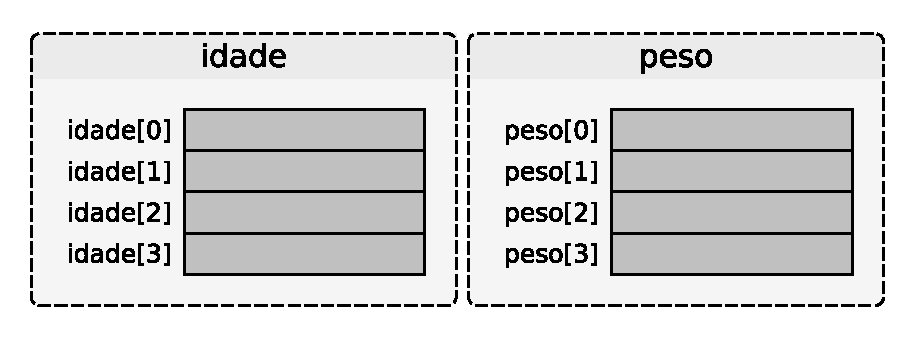
\includegraphics[scale=0.6]{./figures/listas_01.pdf}
     \end{center}
\end{frame}



\begin{frame}[fragile]
\frametitle{Listas}

\begin{minted}[frame=single,  fontsize=\small]{python}
# Cria uma lista ``idade'' com dados inteiros
idade = [21, 25, 36, 78]
# Cria uma lista ``peso'' com números reais
peso = [72.0, 74.5, 88.9, 102.0]
\end{minted}

    \vfill\begin{center}
    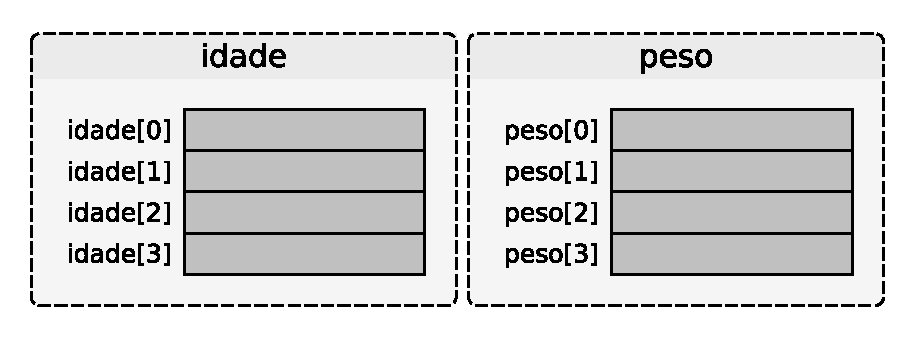
\includegraphics[scale=0.6]{./figures/listas_01.pdf}
    \end{center}


\end{frame}

\begin{frame}[fragile]
    \frametitle{Listas}
    
    \small
    \begin{itemize}
     \item As listas em Python facilitam algumas operações, como:
        
        \begin{itemize}\small
            \item Indexação.
            \item Corte.
            \item Soma.
            \item Multiplicação.
            \item Verificação de membros.
     \end{itemize}

     
    \item \textcolor{red}{O objetivo é agrupar dados para melhorar o acesso lidando com conjuntos dinâmicos}
     
    \item Listas implementam maneiras práticas para:
        \begin{itemize} \small
         \item encontrar o comprimento.
         \item encontrar o maior ou menor elemento.
         \item se um dado existe.
         \item ...
        \end{itemize}
    
    \end{itemize}
\end{frame}

\begin{frame}[fragile]
    \frametitle{Exemplos: listas constantes}
    
    \begin{itemize}
     \vfill \item Python permite que as listas contenham dados de diferentes tipos.
    \end{itemize}

    \vfill \begin{minted}[frame=single,  fontsize=\small]{python}
lista_1 = ['programação', 'circuitos', 1997, 2000];
lista_2 = [1, 2, 3, 4, 5 ];
lista_3 = ["a", "b", "c", "d"];

# print exibe todos os dados das listas
print(lista_1)
print(lista_2)
print(lista_3)
    \end{minted}
    
    
    
    \vfill \begin{minted}[frame=single,  fontsize=\small]{python}
['programação', 'circuitos', 1997, 2000]
[1, 2, 3, 4, 5]
['a', 'b', 'c', 'd']
    \end{minted}
\end{frame}


\begin{frame}[fragile]
\frametitle{Exemplos: indexação}

\begin{itemize}
    \vfill \item Você pode alterar qualquer elemento da lista utilizando o operador [ ].
\end{itemize}

\vfill \begin{minted}[frame=single,  fontsize=\small]{python}
lista_1 = ['programação', 'circuitos', 1997, 2000];

# Podemos alterar itens individuais da lista (indexação)
lista_1[0] = 'gosto de programacao'
print(lista_1)

\end{minted}

\vfill \begin{minted}[frame=single,  fontsize=\small]{python}
['gosto de programacao', 'circuitos', 1997, 2000]
\end{minted}

\end{frame}


\begin{frame}[fragile]
\frametitle{Exemplos: processando todos os itens}

\begin{itemize}
    \vfill \item Usamos o laço \textbf{for} para iterar na lista.
\end{itemize}

\vfill \begin{minted}[frame=single,  fontsize=\small]{python}
lista_1 = ['programação', 'circuitos', 1997, 2000];

# Lê-se: para cada item i em lista_1
for i in lista_1:
    print(i)
print(lista_1)

\end{minted}
    

\vfill \begin{minted}[frame=single,  fontsize=\small]{python}
programação
circuitos
1997
2000
\end{minted}

\end{frame}


\begin{frame}[fragile]
\frametitle{Exemplos: acrescentar}

\begin{itemize}
    \vfill \item Acrescentar um dado no final da lista.
\end{itemize}

\vfill \begin{minted}[frame=single,  fontsize=\small]{python}
a = ["abelha", "zangão"]
print(a)

a.append("formiga")

print(a)
\end{minted}
    

\vfill \begin{minted}[frame=single,  fontsize=\small]{python}
['abelha', 'zangão']
['abelha', 'zangão', 'formiga']
\end{minted}

\end{frame}



\begin{frame}[fragile]
\frametitle{Exemplos: estender}

\begin{itemize}
    \vfill \item Estender uma lista.
\end{itemize}

\vfill \begin{minted}[frame=single,  fontsize=\small]{python}
lista_1 = ['programação', 'circuitos', 1997, 2000];
lista_2 = [1, 2, 3, 4, 5 ];

lista_1.extend(lista_2);

print(lista_1)
\end{minted}
    

\vfill \begin{minted}[frame=single,  fontsize=\small]{python}
['programação', 'circuitos', 1997, 2000, 1, 2, 3, 4, 5]
\end{minted}

\end{frame}



\begin{frame}[fragile]
\frametitle{Exemplos: inserir}

\begin{itemize}
    \vfill \item Inserir um dado.
\end{itemize}

\vfill \begin{minted}[frame=single,  fontsize=\small]{python}
a = ["abelha", "zangão"]
print(a)

# Adiciona na posição 0, início da lista
a.insert(0, "formiga")
print(a)

# Adiciona na posição 2
a.insert(2, "mosca")
print(a)
\end{minted}
    

\vfill \begin{minted}[frame=single,  fontsize=\small]{python}
['abelha', 'zangão']
['formiga', 'abelha', 'zangão']
['formiga', 'abelha', 'mosca', 'zangão']
\end{minted}

\end{frame}


\begin{frame}
 \frametitle{Outros métodos}
 
 \begin{itemize}
    \vfill \item Remover do fim: pop()
    \vfill \item Remover todos os elementos: clear()
    \vfill \item Número de vezes que um elemento aparece na lista: count(x)
    \vfill \item Ordenar: sort()
    \vfill \item Inverter: reverse()
    \vfill \item Comprimento: len(s)
 \end{itemize}
\end{frame}

\begin{frame}{Exercícios}
 \begin{center}
  \includegraphics[scale=0.8]{./figures/man_at_work.png}
 \end{center}
\end{frame}

\end{document}


% 
%
% Local variables section, for Emacs: specifies that this file is the main one.
%
%
%%% Local Variables:
%%% TeX-master: t
%%% End:
